\cotefile{74}
\scanpage{89}
et les \inserted{deux} structures \uline{co} produit obtenues en mettant sur l'un des facteurs une structure de doublet, sur l'autre une structure de segment. Celle en \deleted{\unsure{évidence|induite}} dessinée est
\diagram{\begin{tikzcd}[ampersand replacement=\&,row sep=small,column sep=large]
(ba') \arrow[r,dash] \arrow[dr,dash] \& (bb') \arrow[dl,dash,crossing over]\\
(aa') \arrow[r,dash] \& (ab')
\end{tikzcd}}

On trouve ainsi \uline{les} trois \inserted{uniques} structures de carré sur l'ens à 4 él. produit, \unsure{correspondt|correspondant} aux partitions de cet \uline{ens} de type $(2,2)$\ldots.\par\centerline{\rule{1.1cm}{.4pt}}

Soit un carré $C$, défini par l'ens $C$ de ses sommets, et la partition de type $2,2$, $(C_\alpha)_{\alpha\in\underline D}$ de $C$ en les deux diagonales\inserted{(ou une involution \unsure{ss pt fixe|ss pts fixes|sans pt fixe})}. Une orientation du carré définit, pour chaque $\alpha\in\underline D$.
$\alpha=\{x,x'\}$, une bijection \inserted{$\varphi_\alpha:z\mapsto uz$} de $C_\alpha$ \deleted{$=$} $\{x,x'\}$ sur $C_\beta=\{y,y'\}$. On a $\varphi_\beta\varphi_\alpha=-\mathrm{id}_{C_\alpha}$, $\varphi_\alpha\varphi_\beta=-\mathrm{id}_{C_\beta}$
\diagram{\begin{tikzcd}[ampersand replacement=\&,row sep=small,column sep=small]
x \arrow[r,"\overset{u}{\longrightarrow}"] \arrow[d,dash] \arrow[dr,dash] \& y \arrow[d,dash] \arrow[dl,dash]\\
y' \arrow[r,dash] \& x'
\end{tikzcd}}
(chacune de ces relations impliquant l'autre). D'où
\[
\mathrm{or}(C)\simeq
(\underbrace{\mathop{\bigwedge}_{\alpha\in\underline D} C_\alpha}_{\substack{\underline D^{*}=\text{ens des diagonales}\\\text{du carré dual}}})\wedge\underline D
\simeq \underline D^{*}\wedge\underline D
\]
% archive sheet number: 88

\scanpage{90}
\figure{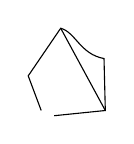
\begin{tikzpicture}[scale=.55]
\draw (0,0)--(-.3,.8)--(.45,1.9) .. controls (.8,1.8) and (.9,1.3) .. (1.45,1.2)--(1.48,0)--(.3,-.12); \draw (.45,1.9)--(1.48,0);
\end{tikzpicture}}
\figure{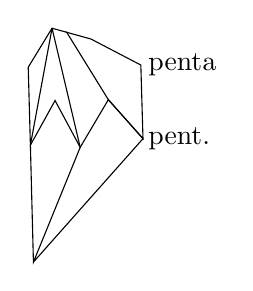
\begin{tikzpicture}[scale=.55]
\draw (0,1.8)--(.55,2.7)--(1.45,2.45)--(2.6,1.85)--(2.65,.15)--(1.85,1.05)--(1.2,-.05)--(.62,1.03)--(.05,0)--(0,1.8);
\draw (.55,2.7)--(.05,0) (.55,2.7)--(1.2,-.05) (.88,2.62)--(1.85,1.05)--(2.65,.15); \draw (.05,0)--(.12,-2.7)--(1.2,-.05) (.12,-2.7)--(2.65,.15);
\node[right] at (2.55,1.85){$\mathrm{penta}$}; \node[right] at (2.55,.15){$\mathrm{pent.}$};
\end{tikzpicture}}
\diagram{\resizebox{\linewidth}{!}{\begin{tikzcd}[ampersand replacement=\&,row sep=1em,column sep=0.65em]

\arrow[from=arc,to=ar,"3"]
\arrow[from=ar,to=seg,"3"]
\arrow[from=arc,to=s,bend left=12]
\arrow[from=dod,to=s,bend right]
\arrow[from=pt,to=s]
\arrow[from=arr,to=db,"2"]
\arrow[from=pt,to=arr]
\arrow[from=car,to=s]
\arrow[from=bp,to=s]
\arrow[from=bp,to=db]
\arrow[from=arr,to=bp]
\arrow[from=cs,to=ca,"2"]
\arrow[from=hs,to=ca,"2"]
\arrow[from=ca,to=car,"2"]
\arrow[from=cs,to=hs,dashed]
\arrow[from=hs,to=car,"\mathrm{car}"]
\arrow[from=hd,to=car,"2"]
\arrow[from=hs,to=htt]
\arrow[from=hdst,to=htt,"2"]
\arrow[from=he,to=cs,"2"]
\arrow[from=he,to=hs,"2"]
\arrow[from=he,to=hdst,"3"]
\arrow[from=he,to=hep]
\arrow[from=he,to=hx,"2"]
\arrow[from=hdst,to=hor,"2"]
\arrow[from=hep,to=hor]
\arrow[from=hs,to=hd,"2"]
\arrow[from=hep,to=hd]
\arrow[from=hor,to=Hsx,"2"]
\arrow[from=hd,to=Hsx,"3"]
\arrow[from=htt,to=Hsx,"2"]
\arrow[from=Hsx,to=s]
\arrow[from=Hsx,to=Hid,"\substack{2\\\mathrm{opp}}"]
\arrow[from=Hid,to=bp]
\arrow[from=Hid,to=H,"3"]
\arrow[from=Hp,to=Hid,"2"]
\arrow[from=HsX,to=Hid,"2"]
\arrow[from=Hsx,to=Htr,"{3\quad u}"]
\arrow[from=He,to=Hsx,"2"]
\arrow[from=hd,to=tri]
\arrow[from=hx,to=hd,"2"]
\arrow[from=hx,to=He,"3"]
\arrow[from=hdst,to=He,"2"]
\arrow[from=tri,to=Htr,"3"]
\arrow[from=Htr,to=H,"\substack{2\\\mathrm{opp}}"]
\arrow[from=HsX,to=H,"2"]
\arrow[from=Hf,to=H,"2"]
\arrow[from=He,to=Htr]
\arrow[from=He,to=HsX,"{2\quad 2}"]
\arrow[from=Hp,to=Ho,"3"]
\arrow[from=HsX,to=Ho,dash]
\arrow[from=Htt,to=Htr,"2"]
\arrow[from=Htt,to=Ho,"2"]
\arrow[from=He,to=Htt,"3"]
\arrow[from=Htt,to=Hf,"2"]
\arrow[from=HsX,to=Hf]
\arrow[from=H,to=TH,"3", "{\deleted{\unsure{\mathrm{triHex}}}\ \deleted{\unsure{(\simeq\mathrm{tripav})}}}"' near end]
\arrow[from=Htr,to=pav,"2"]
\arrow[from=pav,to=TH,"3"]
\arrow[from=bt,to=HsX,dash]
\arrow[from=bt,to=Hid,bend left=9]
 \&  \&  \&  \&  \& |[alias=ca]| \mathrm{Car}_{d*}\simeq\mathrm{pav}+\mathrm{or} \&  \&  \\
 \&  \& |[alias=dod]| \mathrm{dodécép}\simeq\mathrm{pentép}\simeq\mathrm{carrép} \& |[alias=ar]| \substack{\mathrm{Ar}\\{}\simeq\unsure{\mathrm{segpté}|\mathrm{trig\,pt}}} \& |[alias=arc]| \substack{\mathrm{Arc}\\{}\simeq\unsure{\mathrm{segép}|\mathrm{trig\,ép}}} \&  \&  \&  \\
 \&  \&  \& |[alias=seg]| \unsure{\mathrm{seg}}\deleted{\unsure{p}} \&  \&  \&  \&  \\
 \& |[alias=pt]| \mathrm{pent.} \& |[alias=s]| S \&  \&  \& |[alias=car]| \mathrm{car} \&  \& |[alias=cs]| \mathrm{car}_{s*} \\
|[alias=arr]| \unsure{\mathrm{arête}} \&  \&  \& |[alias=htt]| \substack{\mathrm{hex}_{tt*}\\(\simeq\mathrm{pav}+\mathrm{or}\\{}+\mathrm{tria})} \&  \&  \& |[alias=hs]| \substack{\mathrm{hex}_{s*}\simeq\mathrm{car}_{\unsure{t'|r}}\\(\simeq\mathrm{pav}+\mathrm{tria}+\mathrm{or})} \&  \\
|[alias=db]| \substack{\unsure{\mathrm{db\;point}|\mathrm b}\simeq\mathrm{doublet}\\\deleted{\unsure{\mathrm{ob\;arête}}}} \&  \&  \&  \& |[alias=hdst]| \substack{\mathrm{hex}_{\unsure{d*|\Omega*}}\;\deleted{\unsure{b}}\\\unsure{\mathfrak S_3|G_3}} \&  \&  \& |[alias=he]| \substack{\mathrm{hexép}\simeq\mathrm{carép}\\(\simeq\mathrm{pavép})\;(\mathrm G_{\mathrm{pav}})\\(\simeq\mathrm{carép})} \\
 \&  \&  \& |[alias=hor]| \substack{\mathrm{hexor}\\\mathfrak S_3} \&  \&  \& |[alias=hep]| \substack{\mathrm{hexép}'\\(\mathfrak S_3)} \&  \\
|[alias=bp]| \unsure{\mathrm{bi\;pct}|\mathrm{bi\,pt}} \& |[alias=Hid]| \substack{\mathrm{Hex}_{id}^{*}\\(\simeq\mathrm{tria})} \&  \& |[alias=Hsx]| \substack{\mathrm{Hex}_s\simeq\mathrm{hex}\\(\simeq\mathrm{tria})} \&  \& |[alias=hd]| \substack{\mathrm{hex}_{d}\quad\mathfrak S_2\\{}\simeq\mathrm{tria\;pct}\\{}\simeq\mathrm{car}_d} \&  \&  \\
 \&  \& |[alias=Hp]| (\mathbb D_3)\,\mathrm{Hexép}' \&  \&  \&  \&  \&  \\
 \& |[alias=H]| \substack{\mathrm{Hex}\\(\simeq\mathrm{pav})} \&  \& |[alias=Htr]| \substack{(\mathbb D_3)\,\mathrm{Hex}_{tr}\\(\simeq\mathrm{tritria})} \&  \& |[alias=tri]| \mathrm{tria} \&  \&  \\
|[alias=bt]| \unsure{\mathrm{b.}} \&  \& |[alias=HsX]| \substack{\mathrm{Hex}_{s*}\\(\simeq\unsure{\mathrm{bapl}|\mathrm{bapt}|\mathrm{ba\,pt}})} \&  \& |[alias=He]| \substack{(\mathbb D_6)\,\mathrm{Hexép}\simeq\mathrm{hex}_{tr}\\(\simeq\mathrm{trép\,tria})\quad\mathfrak S_3} \&  \&  \& |[alias=hx]| \substack{\mathrm{hex}_{s}\simeq\mathrm{car}_{s}\\(\simeq\mathrm{triaép})\quad\mathfrak S_3} \\
 \&  \&  \& |[alias=Ho]| \mathrm{Hexor} \&  \&  \&  \&  \\
 \&  \& |[alias=Hf]| \substack{\mathrm{Hex}_{t*}\\(\simeq\mathrm{triba})} \&  \& |[alias=Htt]| \substack{\mathrm{Hex}_{tt*}\;(\mathbb F_2\times\mathbb F_2)\\(\simeq\mathrm{trortria})} \&  \&  \&  \\
 \& |[alias=TH]| \substack{\mathrm{triHex}\\(\simeq\mathrm{tripav})} \&  \& |[alias=pav]| \mathrm{pav} \&  \&  \&  \& 
\end{tikzcd}}}
% slanted
\margin{\unsure{investiguer|inventorier|invariants} cube et hypercube dans \unsure{domaine|divers domaines|domaines} \deleted{\unsure{questions}} polyèdres et polyt. \unsure{prod.|pro\ldots}}
\[
\left(\mathrm{prismes}\ \left\{\begin{array}{l}
\text{triangulaires}\\\text{pentagonaux}\\\text{hexagonaux}
\end{array}\right.\right.
\]
produit de polygones\ldots
\figure{\begin{tikzpicture}[x=8mm,y=5mm]\draw[->] (4,2.2) to[bend right=25] (0,0);\draw[->] (4.8,1.7) to[bend left=38] (1,-.9);\end{tikzpicture}}

% slanted
\margin{\tikz[baseline=(a.base)]{\node (a){étranges !};\draw (a.center) ellipse (1.1cm and .34cm);}}
\diagram{\begin{tikzcd}[ampersand replacement=\&,row sep=1.0em]
{} \arrow[d] \& {} \arrow[l] \& {}\\
\bullet \& {} \arrow[ul] \& {} \arrow[ul]\\
{} \& \circ \arrow[ul,dashed] \arrow[uu] \arrow[dd] \& {}\\
{} \& {} \& {} \arrow[uu] \arrow[ul,dash] \arrow[dd]\\
{} \& \bullet \arrow[uuul] \& {}\\
{} \& {} \& {} \arrow[ul]
\end{tikzcd}}
\figure{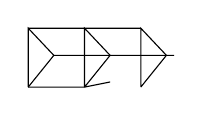
\begin{tikzpicture}[scale=.65]
\foreach \x in {0,1.1,2.2}{\draw (\x,0)--(\x,1.15)--(\x+.5,.62)--(\x,0);}
\draw (0,1.15)--(2.2,1.15) (0,0)--(1.1,0)--(1.6,.1) (.5,.62)--(2.85,.62);
\end{tikzpicture}}
\figure{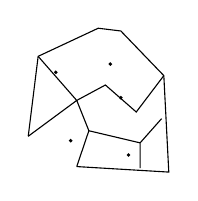
\begin{tikzpicture}[scale=.7]
\draw (0,0)--(.18,1.45)--(1.27,1.96)--(1.68,1.91)--(2.46,1.1)--(2.55,-.65)--(.88,-.55);
\draw (.18,1.45)--(.88,.65)--(1.1,.1)--(.88,-.55) (0,0)--(.88,.65)--(1.4,.93)--(1.96,.44)--(2.46,1.1) (1.1,.1)--(2.03,-.12)--(2.42,.32) (2.03,-.12)--(2.03,-.58);
\foreach \p in {(.5,1.16),(1.49,1.31),(1.68,.7),(.77,-.08),(1.82,-.34)}\fill \p circle(1pt);
\end{tikzpicture}}
% archive sheet number: 89

\scanpage{91}
\diagram{\resizebox{\linewidth}{!}{\begin{tikzcd}[ampersand replacement=\&,row sep=1em,column sep=0.65em]

\arrow[from=cda,to=car,"2"]
\arrow[from=cst,to=cda]
\arrow[from=ho,to=cda,"2"]
\arrow[from=ho,to=hor,"3"]
\arrow[from=hor,to=h,"2"]
\arrow[from=hto,to=hor,"2"]
\arrow[from=hto,to=hb]
\arrow[from=hb,to=h]
\arrow[from=hd,to=h,"3"]
\arrow[from=hto,to=ht,"2"]
\arrow[from=hd,to=car,"2"]
\arrow[from=ho,to=hd,"2"]
\arrow[from=ep,to=cst]
\arrow[from=ep,to=ho,"2"]
\arrow[from=hsx,to=ho,dashed]
\arrow[from=ep,to=hto,"3"]
\arrow[from=ep,to=hsx]
\arrow[from=hsx,to=hd]
\arrow[from=ep,to=hs,"2",dash]
\arrow[from=hs,to=hd,"2"]
\arrow[from=hd,to=tp,"3",dash]
\arrow[from=hs,to=ht,"3"]
\arrow[from=ht,to=h,"2"]
\arrow[from=h,to=pc,"3"]
\arrow[from=pc,to=p,"2"]
\arrow[from=ht,to=trot,"3"]
\arrow[from=tp,to=pc,"3"]
\arrow[from=trot,to=pc,"2"]
\arrow[from=hs,to=tor]
\arrow[from=tor,to=tp,"2"]
\arrow[from=tor,to=trot,"3"]
 \&  \&  \& |[alias=cda]| \mathrm{Car}_{d*}\simeq\mathrm{pav}\;\text{à}\;\unsure{\mathrm{trg\,pct}|\mathrm{trig\,pt}} \&  \&  \\
 \&  \&  \&  \&  \& |[alias=cst]| \substack{\mathrm{Car}_{s*}\simeq\mathrm{pav.}\unsure{+|\times}\mathrm{or}\\{}\simeq\mathrm{pav}+\mathrm{trgép}\\\unsure{\mathfrak S_3|G_3}} \\
|[alias=hor]| \substack{\mathrm{hexor}\\{}\simeq\mathrm{triaor}} \&  \&  \&  \& |[alias=ho]| \substack{\mathrm{hex}_{r'}\\{}\simeq\deleted{\unsure{\mathrm{car}}}_{\unsure{t'|r'}}\;\mathfrak S_3\\{}\simeq\mathrm{triaép}} \&  \\
 \&  \&  \& |[alias=car]| \substack{\mathrm{Car}\\{}\simeq\mathrm{pav\,pct}} \&  \&  \\
 \& |[alias=hb]| \mathrm{hex}_{\unsure{b*|tr*}} \&  \& |[alias=hto]| \substack{\mathfrak S_3\;\mathrm{hex}_{tror}\\(\simeq\mathrm{trgép\,triaor})} \&  \& |[alias=ep]| \substack{\mathrm{hexép}\\(\simeq\mathrm{trgép\,triaép})\quad\mathfrak S_2.(\mathfrak S_3\times\mathfrak S_3)\\(\simeq\mathrm{pavép})\simeq(\mathrm{carép})} \\
|[alias=h]| \substack{\mathrm{hex}\\{}\simeq\mathrm{tria}} \&  \&  \&  \& |[alias=hsx]| \mathrm{hex}_{s*} \&  \\
 \&  \&  \& |[alias=hd]| \substack{\mathrm{hex}_d\\(\simeq\mathrm{car}_d)\\{}\simeq\mathrm{tria}\deleted{\unsure{\mathrm{pé}}}\mathrm{pct}} \&  \&  \\
 \&  \& |[alias=ht]| \substack{\mathrm{hex}_{\unsure{tt|tr}}\\\mathfrak S_3\simeq\mathrm{trgép\,tria}} \&  \&  \& |[alias=hs]| \substack{\mathrm{hex}_s\\{}\simeq\mathrm{triaép}\quad\mathfrak S_3} \\
|[alias=pc]| \substack{\mathrm{Pavcoor}\\{}\simeq\mathrm{trgtria}} \&  \&  \& |[alias=tp]| \substack{\mathrm{trg\,tria\,pct}\\{}\simeq\mathrm{tria}} \&  \&  \\
|[alias=p]| \mathrm{Pav} \&  \& |[alias=trot]| \mathrm{trgortria} \&  \&  \& |[alias=tor]| \mathrm{triaor}
\end{tikzcd}}}
\figure{\begin{tikzpicture}[x=1cm,y=.5cm]\draw (0,1) .. controls (.5,1.05) and (1.15,1.55) .. (1.65,2);\draw (6,-.2) .. controls (6.05,-.52) and (6.3,-.7) .. (6.66,-.75);\end{tikzpicture}}
% archive sheet number: 90

\scanpage{93}
Complexes cubiques généralisés -- (Complexes \uline{triadiques} ou \uline{trialitaires} ?)

$S$ graphe strict, $A\subset\unsure{\mathcal P|\mathfrak P}_2(S)$ l'ens des arêtes. On \deleted{\illegible{1}} appelle \uline{triangle} de $S$ tout $\underline t\in\mathcal P_3(A)$ tel que $x,y\in\underline t$, $x\ne y$ implique que $x,y$ sont ``liés'' (i.e. $\{x,y\}\in A$). Soit $T$ l'ens des triangles de $S$

\uline{Axiome} 1 \quad $\forall\,a\in A,\quad\exists!\,\underline t\in T$ tel que $a\subset\underline t$

\uline{Axiome} 2 \quad $\forall\,\underline t\in T$, $\deleted{\unsure{a}}s\in S\setminus\underline t$, $s$ est lié à un élément de $t$ (unique d'après l'axiome 1\unsure{)|,|).}

\uline{NB} La conjonction de 1 et 2 s'énonce aussi
\[
\uline{\text{Axiome (C)}}\left\{\begin{aligned}
&\text{a) toute arête est contenue dans un triangle}\\
&\text{b) }\forall\,\underline t\in T,\ s\in S\setminus\underline t,\quad\exists!\,s'\in t\ \text{tel que }s\text{ lié}\\
&\quad \text{à }s'\ (\text{i.e. }\{s,s'\}\in A).
\end{aligned}\right.
\]

Pour l'instant on suppose seulement \textcircled{1} \uline{l'axiome 1 vérifié}. Supposons $A\ne\varnothing$ (sinon l'axiome 1 est vide !) donc (grâce à l'axiome 1) $T\ne\varnothing$. Soit $t_0\in T$, \inserted{on posera parfois} $t=\{a,b,c\}$, avec $a,b,c\in \deleted{\unsure{B}}S$.

On supposera de plus pour l'instant que \textcircled{2} \uline{l'axiome 2 est vérifié pour ce $t_0$}, i.e. tt élément de $S\setminus t_0$ est lié à un des él. $a,b,c$\inserted{(unique par l'axiome 1)}. Si $a\in t$, on désigne par $\widetilde E_a$ l'ens de $S\setminus t_0$ liés à $a$. Donc si $t=\{a,b,c\}$ on a bij. can.
\[
S\setminus t_0=\deleted{\unsure{\widetilde E_\alpha}}\coprod_{\alpha\in t_0}\widetilde E_\alpha
\simeq\overline E_a\amalg\overline E_b\amalg\overline E_c
\tag*{\deleted{\unsure{(1)}}}
\]
donc bij can
\[
S\simeq t_0\amalg\coprod_{\alpha\in t_0}\widetilde E_\alpha
\tag*{(1)}
\]

\deleted{D'autre part,}
% archive sheet number: 92

\scanpage{94}
Les arêtes $\subset t_0$ seront appelées horizontales \deleted{\unsure{basiq.|basiques}}basiques, celles qui lient des él. de $t_0$ à des él. de $S\setminus t_0$ sont appelées verticales, celles qui relient des pts de $S\setminus t_0$ sont appelées horizontales supérieures. \deleted{Il y a \unsure{corresp.|exactement}} L'ens des \deleted{\unsure{Prop. 1|Respectivt|Rappel}} arêtes basiques est $\simeq\unsure{\mathcal P|\mathfrak P}_2(t_0)$, l'ens des arêtes verticales est $\simeq\coprod_{\alpha\in t_0}\widetilde E_\alpha$ (\deleted{\unsure{pour}} à $s\in\widetilde E_\alpha$ correspond l'arête verticale $\{s,\alpha\}$).

Exprimons l'axiome 1 pour les arêtes envisagées jusqu'à présent (celles qui ne sont pas hor. sup.). Pour une arête horizontale inférieure, il est déjà exprimé par le fait que les $\widetilde E_\alpha$ $(\alpha\in t_0)$ sont mutuellement disjoints, i.e. par l'écriture $(\underline{1})$. Pour une flèche verticale $\{\alpha,s\}$ $(\alpha\in t_0,s\in S\setminus t_0)$, celà s'exprime ainsi :

\diagram{\begin{tikzcd}[ampersand replacement=\&,row sep=small,column sep=small]
s\arrow[r,dash]\arrow[dr,dash] \& s'\arrow[d,dash]\\
{} \& a\\
{\cdot\, b} \& {\cdot\, c}
\end{tikzcd}}
\noindent\vrule\hspace{.5em}\begin{minipage}{.89\linewidth}\uline{Prop. 2}\quad $\deleted{\unsure{\forall}}\forall\alpha\in t_0$, et $\forall s\in\overline E_\alpha$, $\exists!\,s'\in\overline E_\alpha$ lié à $\alpha$.\end{minipage}

\noindent\vrule\hspace{.5em}\begin{minipage}{.89\linewidth}\uline{Cor}. \quad $\alpha\longrightarrow\alpha'$ est une involution ss pt fixe de $\widetilde E_\alpha$, notée $\sigma_\alpha$. On dénote par $\sigma$ l'application $S\longrightarrow S$ telle que
\[
\sigma\mid t_0=\mathrm{id}_{t_0},\qquad
\sigma\mid\widetilde E_\alpha=\sigma_\alpha\quad\text{pour }\alpha\in t_0.
\]
\end{minipage}
% archive sheet number: 93

\scanpage{95}
Les arêtes (\deleted{\unsure{supé|supér}} horizontales supérieures) de la forme $\{s,\sigma_\alpha(s)\}$ sont appelées supérieures internes (ou supérieures triviales) -- ce sont celles qui lient des pts d'un $=$ $\widetilde E_\alpha$ $(\alpha\in t_0)$. Exprimons l'axiome 1 pour ces nouvelles flèches, on trouve

\noindent\vrule\hspace{.5em}\begin{minipage}{.89\linewidth}\uline{Prop 2} \quad Soit $s,s'\in\widetilde E_\alpha$ $(\alpha\in t_0)$, $s$ \deleted{\unsure{et}} $s'$ liés (i.e. $s'=\sigma_\alpha s$). Soit $\beta\in t_0$, $\beta\ne\alpha$, et soit $t\in\widetilde E_\beta$. Alors $t$ ne peut être lié simultanément à $s$ et $s'$.\end{minipage}

On appellera \deleted{flèches}\inserted{arêtes} (hor.) sup transverses les \deleted{flèches}\inserted{arêtes} (hor) sup qui ne sont pas internes, i.e. qui \deleted{ne sont} relient un pt d'un $\overline E_\alpha$ à un pt d'un $\widetilde E_\beta$ $(\alpha\deleted{\unsure{\ne}}\unsure{,}\beta\in t_0,\ \alpha\ne\beta)$. Soit $\{s,t\}$ $(s\in\overline E_\alpha,\ t\in\widetilde E_\beta)$ une telle arête, \deleted{\unsure{L'existence de}} \inserted{considérons un} \deleted{le} triangle \deleted{correspondant (par l'axiome 1),} \inserted{$\{s,t,u\}$ la contenant ($\exists$ par} \deleted{\unsure{supposé pour le}} l'axiome 1), mais peu importe pour le moment). Évidemt $u\notin t_0$ (car si on avait $u\in t_0$ on \deleted{devrait} aurait $u=\alpha$ et $u=\beta$, or $\alpha\ne\beta$ !) donc $u\in S\setminus t_0=\widetilde E_\alpha\amalg\widetilde E_\beta\amalg\overline E_{\unsure{\gamma|\alpha}}$. On ne peut avoir $u\in\overline E_{\unsure{a|\alpha}}$, car on aurait alors $u=\sigma_\alpha(s)=s'$ par Prop 1, ce qui contredit prop. 2. Pour la $=$ raison on \deleted{\unsure{doit}} a $u\notin\overline E_\beta$, donc $u\in\widetilde E_{\unsure{\gamma|\sigma}}$, i.e.
% archive sheet number: 94

\scanpage{96}
\uline{Prop.} 3 \quad Si $t$ est un triangle contenant une arête Sup. transverse (i.e. contient un pt d'un $\widetilde E_\alpha$ et un d'un $\widetilde E_\beta$, avec \inserted{$\alpha,\beta\in t_0$} $\alpha\ne\beta$) alors les trois arêtes sont transverses, et la relation entre $\alpha\in t_0$ et $s\in t$ : ``$\alpha$ est lié à $s$ (i.e. $s\in\widetilde E_\alpha$)'' est une bijection $t_0\xrightarrow{\sim}t$.

Les triangles en question s'appellent triangles supérieurs, leur \unsure{2} ens est noté $\deleted{\unsure{\widetilde T}}\widetilde\Gamma$. On a donc des applications
\[
\deleted{\unsure{\widetilde T}}\widetilde\Gamma\xrightarrow{\widetilde\varphi_\alpha}\widetilde E_\alpha\qquad(\alpha\in t)
\]
(ou encore
\diagram{\begin{tikzcd}[ampersand replacement=\&]
\overline E_a\& {}\&\widetilde E_b\\
{}\&\widetilde\Gamma\arrow[ul,"\overline\varphi_a"]\arrow[ur,dash,"\widetilde\varphi_b"']\arrow[d,"\widetilde\varphi_c"]\&{}\\
{}\&\widetilde E_c\&{}
\end{tikzcd}}
) \deleted{définissant}\inserted{\unsure{équivaut à|équivalant à|équivalentes à}} une application unique
\[
\widetilde\Gamma\xrightarrow{\widetilde\varphi}\prod_{\alpha\in t_0}\widetilde E_\alpha
\qquad(=\widetilde E_c\times\widetilde E_b\times\overline E_c),
\]
L'axiome 1 pour les arêtes sup. transverses équivaut alors à la

\uline{Prop.} 4 \quad Si $\deleted{\alpha,\beta\in t_0,\ \alpha=}u\in\unsure{\mathcal P|\mathfrak P}_2(t_0)$ est une
% archive sheet number: 95

\scanpage{97}
arête basique \inserted{(disons $\unsure{a|u}=\{\alpha,\beta\}$)}, l'application
\[
\widetilde\Gamma\xrightarrow{\widetilde\varphi_u}\prod_{i\in u}\widetilde E_i
\quad(\simeq\widetilde E_\alpha\times\widetilde E_\beta)
\]
est \uline{injective}, et son image est formée des \deleted{\unsure{toutes|tous}} les \deleted{familles} couples $(s,t)\in\widetilde E_\alpha\times\widetilde E_\beta$ tels que $s$ soit lié à $t$.

\uline{Scholie} En résumé, moyennant les conditions \textcircled{1} et \textcircled{2} plus haut, on voit que la structure de graphe $S$, muni du triangle $t_0$, se reconstitue à partir de la donnée de

a) un ens $t_0$ tel que $\operatorname{Card}t_0=3$

b) une famille $\deleted{\unsure{E|\widetilde E}}F=(\widetilde E_\alpha)_{\alpha\in t_0}$ d'ens. \inserted{munis chacun d'une invol. $\sigma_\alpha$ ss pt fixe}

c) une partie $\widetilde\Gamma\lhook\joinrel\xrightarrow[\widetilde\varphi]{}\underbrace{\prod_{\alpha\in t_0}\widetilde E_\alpha}_{\text{\textquotedbl}\widetilde p}$

[satisfaisant les conditions

$\alpha$) $\forall u\in\unsure{\mathcal P|\mathfrak P}_2(t_0)$, l'application $\widetilde\Gamma\xrightarrow{\widetilde\varphi_u}\prod_{\alpha\in u}\widetilde E_\alpha$ est injective,

\inserted{(\unsure{**}) Si $\alpha,\beta\in t_0$, $\alpha\ne\beta$, et si $s\in\widetilde E_\alpha$, $t\in\widetilde E_\beta$, si $(s,t)\in\mathrm{Im}\,\widetilde\varphi_{\{\alpha,\beta\}}(\widetilde\Gamma)$ alors $(\sigma_\alpha s,t)\notin\mathrm{Im}\,\widetilde\varphi_{\{\alpha,\beta\}}(\widetilde\Gamma)$}
% margin note written sideways
\margin{$\boxed{**}$ Si $(s_\alpha)_{\alpha\in\underline t_0}\in\prod_{\alpha\in\underline t_0}\widetilde E_\alpha$ \deleted{est tel que} \deleted{\unsure{$\forall\alpha$ si}} $(\underline t_\alpha)_{\alpha\in\underline t_0}\in{\unsure{\widetilde T|\widetilde\Gamma}}^{\underline t_0}$ sont tels que \deleted{\unsure{$\forall$}} $\alpha,\beta\in\underline t_0$, $\alpha\ne\beta$ on a $s_\beta=\varphi_\beta(\underline t_\alpha)$, alors les $\underline t_\alpha$ sont égaux}

de la façon suivante

\[
S\simeq t_0\amalg\coprod_{\alpha\in t_0}\widetilde E_\alpha \tag*{$1^\circ$)}
\]
\[
2^\circ)\ \deleted{\text{deux pts}}\ \left\{\begin{aligned}
&\alpha)\ \text{Deux pts de }t_0\text{ sont liés}\\
&\beta)\ \text{un point de }\widetilde E_\alpha\text{ est lié à un et un}\\
&\quad\text{seul él. de }t_0,\ \text{savoir }\alpha\quad(\text{si }\alpha\in t_0)\\
&\unsure{\gamma) }\text{un point }s\text{ de }\overline E_\alpha\text{ est lié à un }\inserted{\text{et un}}\text{ seul pt de}\\
&\quad\unsure{\text{lui}|\widetilde E_\alpha},\ \text{savoir }\sigma_\alpha(s)\\
&\delta)\ \deleted{\text{Soit}}\ \alpha,\beta\in t_0,\ \alpha\ne\beta,\quad s\in\widetilde E_\alpha,\ t\in\overline E_\beta,\quad\text{alors }s,t\text{ sont}
\end{aligned}\right.
\]
% archive sheet number: 96

\scanpage{98}
liés sss $(s,t)\in\mathrm{Im}\,\varphi_{\{\alpha,\beta\}}(\widetilde\Gamma)$.

Étant donné des données a) b) c), satisfaisant la condition $(\alpha)$, le graphe qu'on vient de décrire satisfait les conditions \textcircled{1} (Axiome 1) et \textcircled{2} (L'axiome 2 pour le \inserted{seul} triangle $t_0$). L'ens \inserted{$T$} des triangles de $(S,A)$ est alors donné, mod bijection, par
\[
T\simeq\underbrace{\{t_0\}}_{\substack{\text{triangle}\\\text{de base}}}\amalg
\underbrace{\coprod_{\alpha\in t_0}E_\alpha}_{\substack{\text{triangles}\\\text{verticaux}}}\amalg
\underbrace{\widetilde\Gamma}_{\substack{\text{triangles (horiz.)}\\\text{supérieurs}}}
\]
où on pose \deleted{\unsure{$E$}}
\[
E_\alpha=\widetilde E_\alpha/\sigma_\alpha
\]
(de sorte que $\widetilde E_\alpha$ est un rev. de degré 2 de $E_\alpha$). Pour $\alpha\in t_0$, un élément $u$ de $E_\alpha$, i.e. $u\in\unsure{\mathcal P|\mathfrak P}_2(\widetilde E_\alpha)$ formé d'une orbite sous $\sigma_\alpha$, \unsure{son|le} triangle \inserted{(vertical)} associé est par définition \deleted{\unsure{$\{$}}$u\unsure{\amalg|\cup}\{\alpha\}$. Pour $\deleted{\unsure{\gamma\in\widetilde\Gamma}}\tau\in\widetilde\Gamma$, le triangle associé est par définition l'ens \deleted{\unsure{des}} $\{\varphi_\alpha(\tau)\}_{\alpha\in t_0}$.

\inserted{Rien n'empêche pour l'instant qu'on ait $\widetilde\Gamma=\varnothing$ ! Mais} On se propose maintenant d'exprimer l'axiome 2 pour \uline{ts} les triangles de $S$ (pas seulement $t_0$). Prenons d'abord les
% archive sheet number: 97

\scanpage{99}
Cas des triangles \uline{verticaux} $\{\alpha,s,s'\}$ $(\alpha\in t_0,s\in\widetilde E_\alpha,s'=\sigma_\alpha(s))$ On trouve

\uline{Prop 5} \quad Soient $\alpha\in\unsure{t|t_0}$, $s,s'$ deux arêtes liées de $E_\alpha$, et $\deleted{\beta\in t_0,\ \beta\ne\unsure{\beta|\alpha},}$ $t\in\widetilde E_\beta$, avec $\beta\in t_0$, $\beta\ne\alpha$, alors $t$ est lié à \deleted{au plus} $s$ ou à $s'$ (\uline{NB} par prop. 2, ou \unsure{rien que sous|si on veut par|encore suivant} la condition $(\alpha)$, \deleted{il est lié à un} il n'est pas lié à $s$ \uline{et} à $s'$, donc il est lié à un et un seul des deux pts $s,s'$). En termes des données du Scholie : Soit $\widetilde\Gamma_{\alpha,\beta}\subset\widetilde E_\alpha\times\widetilde E_\beta$ l'image de $\widetilde\Gamma$ dans $\widetilde E_\alpha\times\widetilde E_\beta$, soient $s,s'\in\widetilde E_\alpha$, $t\in\widetilde E_\beta$, avec $s'=\sigma_\alpha s$ i.e. $s=\sigma_\alpha s'$. Alors on a $\{s,t\}\in\unsure{\widetilde E_{\alpha\beta}|\widetilde\Gamma_{\alpha\beta}}$ ou $\{s',t\}\in\widetilde\Gamma_{\alpha\beta}$

\noindent\vrule\hspace{.5em}\begin{minipage}{.89\linewidth}\uline{Cor} \quad \deleted{\unsure{Alors}} Sous les conditions précédentes, posant $t'=\sigma_\beta t$, si \inserted{$s,t$ liés i.e.} $\deleted{(s,t)\in\unsure{\Gamma|\widetilde\Gamma}}\ \{s,t\}\in A$ i.e. $(s,t)\in\widetilde\Gamma_{\alpha\beta}$, alors \inserted{$s',t'$ liés i.e.} $\{s',t'\}\in A$ i.e. $(s',t')\in\widetilde\Gamma_{\alpha\beta}$.

\end{minipage}

En effet, $t'$ étant lié à $s$ ou $s'$, et ne pouvant être lié à $s$ (car $s$ serait lié à $t$ et $t'$ en opposition à prop 2) il est lié à $s'$.

\noindent\vrule\hspace{.5em}\begin{minipage}{.89\linewidth}\uline{Cor} \quad Soit $\deleted{\unsure{\sim}}\sigma_{\widetilde p}=\prod_{\alpha\in t_0}\deleted{\unsure{\alpha}}\overline\sigma_\alpha$ l'autom \inserted{\unsure{inv.}} d'ordre 2 (ss pt fixe) de $\prod\widetilde E_\alpha$. Alors $\widetilde\Gamma$ est stable par $\unsure{\ll|\sim}\sigma_{\widetilde p}\unsure{\gg|{>}}$\unsure{?|\textquoteright|;}\end{minipage}

On note $\sigma_{\widetilde\Gamma}$ l'autom d'ordre 2 de $\widetilde\Gamma$ induit par $\sigma_{\widetilde p}$.
% archive sheet number: 98

\scanpage{100}
\uline{Cor} \quad Soit\deleted{\unsure{nt}} $\alpha\in t_0$, $s\in\overline E_\alpha$, alors si $\deleted{\beta,\gamma\in t_0\setminus\{\alpha\},\ \unsure{\beta}\ne\beta,\ \beta\ne\gamma}\deleted{\unsure{\in t_0,\ \beta\ne\alpha}}\beta\in t_0\setminus\{\alpha\}$ l'ens $\widetilde E_\beta(s)$ \inserted{$\subset\overline E_\beta$} des $t\in\widetilde E_\beta$ \deleted{\unsure{$t$}} liés à $s$ est une \uline{section} de $\widetilde E_\beta$ sur $E_\beta=\widetilde E_\beta/\sigma_\beta$. Soit \inserted{de $=$} $\overline{\unsure{a|\gamma}}\deleted{\ne\alpha,\ \ne\beta}\inserted{\in\unsure{\widetilde t|t_0}\setminus\{\alpha,\beta\}}$, $(\gamma\ne\beta)$, d'où $\overline E_\gamma(s)$ section de $\widetilde E_\gamma$ sur $E_\gamma$, la relation entre $t\in\widetilde E_\beta(s)$ et $t'\in\widetilde E_\gamma(s)$ ``$t$ et $t'$ sont liés i.e. $(t,t')\in\widetilde\Gamma_{\beta,\gamma}$'' est une bijection \deleted{entre $\widetilde E_\beta(s)$ et}
\[
u_s^{\gamma,\beta}:\widetilde E_\beta(s)\xrightarrow{\sim}\widetilde E_\gamma(s)
\]

\uline{Cor} \quad Si \deleted{\unsure{on|Si}} $\widetilde E_\alpha\ne\varnothing$, alors $\operatorname{Card}\deleted{\unsure{\sim}}E_\beta=\operatorname{Card}E_\gamma$ donc $\operatorname{Card}\widetilde E_\beta=\operatorname{Card}\widetilde E_\gamma$ ; si ce \deleted{\unsure{dernier}} cardinal est $\ne0$ i.e $\widetilde E_\beta\deleted{\unsure{E_\gamma}}\ne\varnothing$ $(\deleted{\unsure{\longleftarrow|\longleftrightarrow}}\Longleftrightarrow\widetilde E_\gamma\ne\varnothing)$. Alors $\widetilde E_\alpha,\widetilde E_\beta,\widetilde E_\gamma$ ont $=$ cardinal (et de $=$ $E_\alpha,E_\beta,E_\gamma$ ont $=$ cardinal).

\uline{NB} \inserted{\unsure{$\times$}}Évidemt, si $\widetilde E_\alpha=\varnothing\quad\forall\alpha\in t_0$, les axiomes \deleted{\unsure{envisagés}} 1 et 2 sont trivialemt satisfaits. De $\overline{\mathrm m}$ si $\widetilde E_\alpha\ne\varnothing$, et $\widetilde E_\beta,\widetilde E_\gamma=\varnothing$ (donc $\widetilde\Gamma=\varnothing$, donc pas d' \deleted{flèches} arêtes sup transverses). Alors \inserted{le graphe} $S$ est \deleted{\unsure{formé}} de la forme
\[
S=\{\alpha\}\amalg\widetilde S'\deleted{\unsure{a}}\qquad\text{où }\widetilde S'=S-\{\alpha\}
\]
est muni d'une invol. $\sigma_{S'}$ sans pt fixe, et les arêtes sont les $\{\alpha,s\}$ $(s\in S')$ et les $(s,\sigma_{S'}s)$ $(s\in\widetilde S')$, donc
\[
A\simeq\widetilde S'\amalg\underbrace{\widetilde S'/\sigma_{S'}}_{S'}.
\]
\deleted{\unsure{Ma|Mais}}
% archive sheet number: 99

\scanpage{101}
On supposera dorénavant qu'on a \deleted{l'axi.}

\noindent\vrule\hspace{.5em}\begin{minipage}{.89\linewidth}\uline{Axiome 3} \quad Les $\widetilde E_\alpha$ $(\alpha\in t_0)$ sont $\ne\varnothing$, i.e. on n'est pas dans le cas \inserted{(trivial)} envisagé dans la NB précédente, $\unsure{\Leftrightarrow|{=}}$ ou encore : par tt sommet $s\in S$ passent au moins 2 triangles.\end{minipage}

Il reste exprimer dans ce cas, l'axiome 2 pour les triangles sup. Or il est automatique !

\diagram{\begin{tikzcd}[ampersand replacement=\&,row sep=.5em,column sep=.5em]
{}\& s\arrow[dl,dash]\arrow[dr,dash]\arrow[dd,dash]\&{}\\
t\arrow[rr,dash]\arrow[dd,dash]\&{}\&u\arrow[dd,dash]\\
{}\&a\arrow[dl,dash]\arrow[dr,dash]\&{}\\
b\arrow[rr,dash]\&{}\&c
\end{tikzcd}}
\deleted{\uline{Prop} 6 \quad Soit $\{s,t,u\}$ sur $\{a,b,c\}=t_0$ un triangle supérieur (i.e. un $t\in\widetilde\Gamma$), et soit $s_1\in\overline E_a\setminus\{s,s'=\sigma_a s\}$. Alors $s_1$ est lié à $t$ ou $u$ (NB bien sûr, pas aux \uline{deux} à la fois\ldots.)}

En effet, \deleted{\unsure{tout}} a) tt $\alpha\in t_0$ est lié à un pt de $\{s,t,u\}$

\deleted{\unsure{$s$ distinct} \unsure{et|de}} b) Si $\deleted{\unsure{a}}s_1\in\deleted{E_\alpha,\ \text{alors}}S\setminus t_0=\coprod\overline E_\alpha$, disons $s_1\in E_a$, \deleted{pour $\alpha\in t_0$ \unsure{conv.}, alors} $s_1\notin t$ i.e. $s_1\ne s$, si $s_1$ \deleted{$=\sigma_\alpha s=s'$, il est} n'est pas lié à $s$ i.e. $s_1\ne s'=\sigma_a s$, montrons qu'il est lié à $t$ ou $u$. En effet, s'il n'était lié à aucun des deux, alors $s'_1=\sigma_\alpha s_1$ serait lié aux deux à la fois, et comme $s'_1\ne s$ c'est absurde.

\par\centerline{\rule{4cm}{.4pt}}

\uline{\unsure{Rescholie|Résolution}}

En résumé, la donnée d'un complexe $(S,A)$ \deleted{\unsure{entier|et \illegible{1}}} satisfaisant les axiomes \textcircled{1}, \textcircled{\unsure{2|1}} et qui n'est pas du type trivial \deleted{\unsure{étudié|étoile}} \inserted{(\unsure{discret|disons}, se réduisant à un triangle, ou à une étoile de triangles
\figure{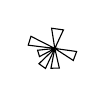
\begin{tikzpicture}[scale=.20]\foreach \a/\b/\r in {65/99/1.3,153/173/1.7,186/208/1.1,224/245/1.4,259/283/1.28,327/352/1.4}{\draw (0,0)--(\a:\r)--(\b:\r)--cycle;}\end{tikzpicture}})} équivaut à celle de
% archive sheet number: 100

\scanpage{102}
a) $t_0$ ens de card 3

b) $\widetilde\Gamma$ ens \inserted{$\ne\varnothing$} avec involution $\deleted{\unsure{\sim}}\sigma_{\widetilde\Gamma}$ (sans pts \unsure{fixe|fixes})

c) Une famille $(\overline E_\alpha)_{\alpha\in t_0}$ de quotients de $\widetilde\Gamma$ \deleted{\unsure{par|plus}}

Avec les conditions suivantes

$\alpha$) Les $\widetilde E_\alpha$ stables par $\deleted{\unsure{\sim}}\sigma_{\widetilde\Gamma}$ (\unsure{donc|soit|sur|dont} $\sigma_\alpha$ induit) et les $\sigma_\alpha$ sont sans pts fixes

$\beta$) $\deleted{\unsure{\widetilde\Gamma\in|\widetilde E}}\forall\alpha,\beta\in t_0,\ \alpha\ne\beta$, l'application
\[
\widetilde\Gamma\xrightarrow{\widetilde\varphi_{\alpha,\beta}}\widetilde E_\alpha\times\widetilde E_\beta
\]
est \uline{injective}, et si $\Gamma_{\alpha\beta}$ est son image, \deleted{on a la condition} et si $u\in\unsure{\mathcal P|\mathfrak P}_2(\widetilde E_\alpha)$ \deleted{sont distincts et conjugués par} \inserted{est une orbite sous} $\sigma_\alpha$ \deleted{$(s\ne s')$} et $t\in\widetilde E_\beta$, on a : $\exists!\,s\in u$ tel que $(s,t)\in\widetilde\Gamma_{\alpha,\beta}$

\inserted{\textcircled{$\gamma$} l'axiome \uline{(**) plus} haut sur $(s_\alpha)_{\alpha\in t_0}$ et $(\underline t_\alpha)_{\alpha\in t_0}$}

\deleted{On peut déduire de $\beta$), posant $\Gamma=\widetilde\Gamma/\sigma_{\widetilde\Gamma}$, $E_\alpha=\widetilde E_\alpha/\widetilde\sigma_\alpha$, que}
\[
\deleted{\Gamma\xrightarrow{\varphi_{\alpha\beta}}{}}
\]

Soit \deleted{\unsure{$E?$}} $\Gamma=\widetilde\Gamma/\sigma_{\widetilde\Gamma}$, $E_\alpha=\widetilde E_\alpha/\sigma_\alpha$, donc on a des quotients $E_\alpha$ de $\Gamma$
\[
\Gamma\xrightarrow{\varphi_\alpha} E_\alpha,\qquad\Gamma\xrightarrow{\varphi}\prod_{\alpha\in t_0}E_\alpha
\]
et l'axiome a) implique que \inserted{$\forall\alpha$,} $\widetilde\Gamma$ s'identifie à l'image inverse des revêtmts d'ordre 2 $\overline E_\alpha$ de $E_\alpha$. Donc la famille de données
% archive sheet number: 101

\scanpage{103}
a) b) c) avec l'axiome $\alpha$ équivaut à : la donnée de l'ens $\Gamma$ \inserted{$\ne\varnothing$}, et de la famille $(E_\alpha)_{\alpha\in t_0}$ de ses quotients
\[
\varphi_\alpha:\Gamma\longrightarrow E_\alpha,\qquad
\varphi:\Gamma\unsure{\text{---}|\longrightarrow}\prod_{\alpha\in t_0}E_\alpha,
\]
\deleted{et}\inserted{puis} des rev. d'ordre 2
\[
\widetilde E_\alpha\xrightarrow{p_\alpha} E_\alpha\qquad(\alpha\in t_0)
\]
et d'un \uline{syst. transitif} de\deleted{\unsure{d}} \inserted{$\Gamma$-}iso. entre les revêtements $\varphi_\alpha^*(\widetilde E_\alpha/E_\alpha)$ de $\Gamma$ (permettant de définir $\widetilde\Gamma$ par identification\ldots) Ceci posé, l'axiome $\beta_{\widetilde\Gamma})$ \deleted{implique}\inserted{équivaut à} l'axiome

$\beta_\Gamma$) Si $\{\alpha,\beta\}\in\unsure{\mathcal P|\mathfrak P}_2(t_0)$, alors
\[
\Gamma\xrightarrow{\varphi_{\alpha\beta}}E_\alpha\times E_\beta
\]
est \uline{bijectif}

La classification de ces ``complexes cubiques généralisés'' \deleted{\unsure{admet}} se décompose donc en deux questions exactement

I) Description des systèmes
\[
\left(\Gamma\xrightarrow{\varphi_\alpha}\Gamma_\alpha\right)_{\alpha\in t_0}
\]
de quotients (\unsure{paramétré|paramétrés} par $t_0$ de card 3) d'un ens $\Gamma\ne\varnothing$, satisfaisant l'axiome $\beta_\Gamma$
% archive sheet number: 102

\scanpage{104}
II) Pour un tel syst$_{\unsure{e}}$ donné, classifier les ``rev. d'ordre 2 \unsure{des diagrammes|du diagramme}
\[
\left(\Gamma\xrightarrow{\varphi_\alpha}\Gamma_\alpha\right)_{\alpha\in t_0}
\]
i.e. \deleted{\unsure{des}} \unsure{des|deux|de tels} diagrammes \inserted{particuliers} de la forme
\diagram{\begin{tikzcd}[ampersand replacement=\&]
E_{\unsure{a|\alpha}}\&{}\&E_c\\
{}\&\Gamma\arrow[ul,"\varphi_a"]\arrow[ur,"\varphi_c"']\arrow[d,"\varphi_\beta"]\&{}\\
{}\&E_\beta\&{}
\end{tikzcd}}
puis ceux qui satisfont l'axiome $(\gamma)=(\unsure{**|\alpha\alpha|\mathrm{Ka}})$

\begin{center}\rule{.36\linewidth}{.35pt}\\[-.4em]\rule{.26\linewidth}{.35pt}\\[-.4em]\rule{.16\linewidth}{.35pt}\end{center}
% archive sheet number: 103

\scanpage{105}
$s\in\widetilde E_a$ définit
\[
\begin{aligned}
\widetilde E_b&\overset{f_{s,b}}{\simeq}E_b\times\{\pm1\}
&\qquad\widetilde E_b&\simeq E\\
\widetilde E_c&\overset{f_{s,\unsure{a|c}}}{\simeq}E_c\times\{\pm1\}
\end{aligned}
\]

\diagram{\begin{tikzcd}[ampersand replacement=\&,row sep=small,column sep=small,execute at end picture={\draw ([xshift=-3mm,yshift=-3mm]tl.south) -- ([xshift=7mm,yshift=5mm]sp.north);}]
\& |[alias=sp]| \deleted{s} \arrow[dl,dash] \arrow[dr,dash] \& {}\\
|[alias=tl]| \deleted{t} \arrow[rr,dash] \& \& \deleted{u}
\end{tikzcd}}
\[
\begin{aligned}
&\deleted{(\unsure{s_1,s'_1|s,s',s'_1})}\quad\deleted{4p^2\quad2p^2}\\
&\hspace{5em}(s_1,s'_1)
\end{aligned}
\]
\[
\begin{aligned}2+2c\\ \deleted{2\deleted{\unsure{\cdot|+}}+2c}\end{aligned}
\]
\diagram{\begin{tikzcd}[ampersand replacement=\&,row sep=0pt,column sep=small,execute at end picture={\draw ([xshift=-1mm,yshift=-1mm]ss.south east)--([xshift=11mm,yshift=11mm]ss.north east);}]
s\arrow[rrd,dash] \&|[alias=ss]| s'\arrow[rrd,dash]\&{}\&{}\\
{}\&{}\&t,\&t'
\end{tikzcd}}

\[
\begin{aligned}
\operatorname{Card} S&=\deleted{\unsure{E|2}}3+6c=3(1+2c)\\
\operatorname{Card}\unsure{\operatorname{Ét}|\operatorname{Et}|E}_S(s)&=2+2c=2(1+c)\\
\operatorname{Card} A&=3(1+c)(1+2c)\\
&=3(1+3c+2c^2)\\
&=3+6c+3c\\
&\qquad+3(2c^2)
\end{aligned}
\]
\diagram{\begin{tikzcd}[ampersand replacement=\&,row sep=small,column sep=small,execute at end picture={
\draw ([xshift=-7mm,yshift=4mm]p.north west)--([xshift=4mm,yshift=-4mm]q.south);
\draw ([xshift=-3mm,yshift=4mm]r.north west)--([xshift=5mm,yshift=-5mm]r.south east);
\draw ([xshift=-2mm,yshift=4mm]e.north west)--([xshift=2mm,yshift=-3mm]e.south east);
\draw ([xshift=2mm,yshift=3mm]e.north east) to[bend left=15] ([xshift=4mm]b.east)--([xshift=2mm,yshift=-2mm]b.south east)--(b.south);
}]
\widetilde\Gamma\arrow[r,dash]\arrow[d]\arrow[rr,bend left=32,dash,"\sim"] \&
|[alias=p]| \deleted{\widetilde E_\alpha\times\widetilde E_\beta}\arrow[r,dash]\arrow[d] \&
|[alias=r]| \deleted{\widetilde E_\alpha\times E_\beta}\arrow[r,dash]\arrow[dl] \&
|[alias=e]| \deleted{\widetilde E_{\deleted{\beta}\alpha}}\arrow[d] \\
\Gamma\arrow[r,dash,"\sim"] \& |[alias=q]| \deleted{E_\alpha\times E_\beta}\arrow[rr,dash]\&{} \&
|[alias=b]| \deleted{E_{\deleted{\beta}\alpha}}
\end{tikzcd}}
\[
\begin{aligned}
\operatorname{Card} T&=\frac13\operatorname{Card} A,\\
&=(1+c)(1+2c)\\
&=\deleted{\unsure{1}}1+3c+2c^2
\end{aligned}
\]
\[
\begin{aligned}
\operatorname{Card} T(s)&=1+c\quad\deleted{\text{si }s\in t_0}\\
\deleted{\operatorname{Card} T(s)=1+c}&\\
\operatorname{Card} T&=\tfrac13\operatorname{Card} S\ (1+c)
\end{aligned}
\qquad
\begin{aligned}
\operatorname{Card}\widetilde\Gamma&=2c^2\\
\operatorname{Card}\Gamma&=c^2\\
\operatorname{Card}\widetilde E_a&=2c\\
\operatorname{Card}E_a&=c
\end{aligned}
\]
\figure{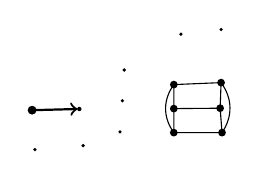
\begin{tikzpicture}[x=6mm,y=5mm]
\fill (0,0) circle (1.6pt) (1,0.03) circle (.8pt) (.06,-1) circle (.65pt) (1.08,-.9) circle (.65pt);
\draw[->,thick] (0,0)--(.96,.03);
\foreach \x/\y in {1.86/-.55,1.91/.24,1.95/1.02,3.15/1.93,4/2.05}{\fill (\x,\y) circle (.65pt);}
\draw (3,0.65)--(4,.7)--(3.98,.05)--(4.02,-.57)--(3,-.57)--cycle;
\draw (3,.04)--(3.98,.05); \draw (3,.65) to[bend right=36] (3,-.57); \draw (4,.7) to[bend left=35] (4.02,-.57);
\foreach \x/\y in {3/.65,4/.7,3/.04,3.98/.05,3/-.57,4.02/-.57}{\fill (\x,\y) circle (1.4pt);}
\end{tikzpicture}}
% archive sheet number: 104
